\hfour{Datenbankservice}

\begin{figure}[H]
    \centering
    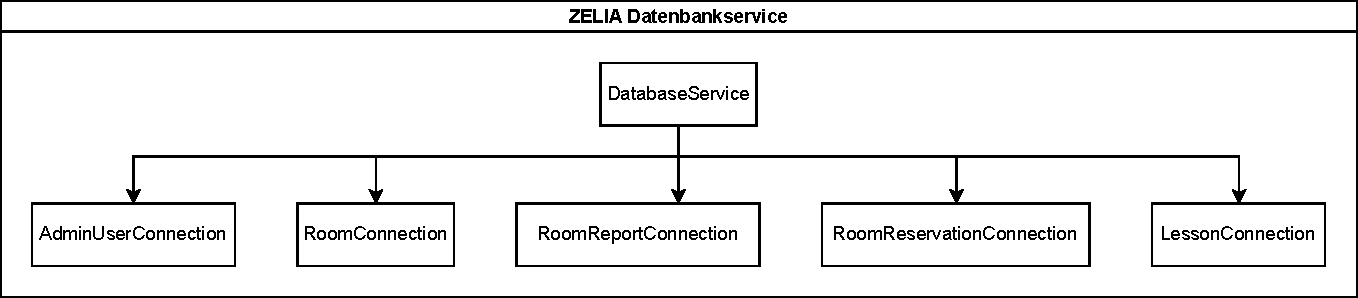
\includegraphics[width=\textwidth]{media/Sequelize/DatabaseService.svg.pdf}
    \caption{Abhängigkeiten des Datenbankservice}
\end{figure}

Durch die verschiedenen Verbindungsklassen wird ein direkter Zugriff auf die Datenbank und die Tabellen in ihr ermöglicht. Der Datenbankservice ist nun für die Kommunikation mit dem restlichen Server zuständig. 

Das Ziel hinter diesem eigenen Services war es, die Interaktion des restlichen Servers mit der internen Datenbankkommunikation so gering wie möglich zu halten. Durch den externen Service muss nur dieser aufgerufen werden. Der Datenbankservice übernimmt ab diesem Zeitpunkt die gesamte Aufrufhierarchie der Datenbank.

Außerdem wird über den Datenbankservice das Auftreten von Fehlern gehandhabt. Beispielsweise wird überprüft, ob die Datenbank verfügbar ist, oder ob beim Verbindungsaufbau etwas nicht geklappt hat, oder der ausgewählte Raum in der Datenbank nicht vorhanden ist. Dies wird über verschiedene "Exceptions" realisiert, welche einerseits den Entwicklern beim Programmieren helfen die Übersicht zu behalten und andererseits den Benutzer*innen im fertigen Produkt ein Feedback liefern, ob ihre Aktion erfolgreich war, oder nicht.

Beispiel für eine Exception:

\typescript{code/Sequelize/exception.ts}{Datenbank nicht verfügbar Exception}

Je nachdem, welche Aktion vom Server angefragt wird muss ein Parameter mitgegeben werden oder nicht. Wenn ein Parameter mitgegeben wird, wird dieser in die gewünschte Zugriffsmethode weitergereicht.

\typescript{code/Sequelize/all.ts}{Beispiel für eine Datenbankservicemethode}